\documentclass[multicolumn, 12pt]{extarticle}
\usepackage[english]{babel}
\usepackage{NotesTeX}
\usepackage{subfigure}
\usepackage{tikz}
\usetikzlibrary{arrows}
\usepackage{multirow}
\usepackage{listings}
\usepackage{extarrows}
\usepackage{parskip}
\usepackage{eurosym}
\usepackage{footmisc}
\usepackage{kantlipsum}
\usepackage{algorithm}
\usepackage{algpseudocode}

\usepackage{titlesec}

\setcounter{secnumdepth}{4}

\renewcommand{\deg}{^{\circ}}
\newcommand\numberthis{\addtocounter{equation}{1}\tag{\theequation}}
\newcommand{\hksqrt}[2][]{\ \mathpalette\DHLhksqrt{[#1]{#2\,}}}
\def\DHLhksqrt#1#2{\setbox0=\hbox{$#1\sqrt#2$}\dimen0=\ht0
    \advance\dimen0-0.3\ht0
    \setbox2=\hbox{\vrule height\ht0 depth -\dimen0}
    {\box0\lower0.65pt\box2}}

\onecolumn

\graphicspath{{../plots/}}
%\collaborationImg{
\includegraphics[width=30mm]{UIO.png}}

\author{\Large Sara Pernille Jensen \& Håkon Olav Torvik}
\title{\Huge P3: We did a thing}
\affiliation{\large FYS-STK4155 – Applied Data Analysis and Machine Learning
\\Autumn 2021\\Department of Physics\\University of Oslo\\\\\today}
\begin{document}
\abstract{
	The very concrete abstract.
}

% Ting til gjennomlesning:
% ingen kolon før likning med mindre nødvendig
% tegnsetting i likninger skal være som i normal tekst
% Tror det står algorithms noen steder det egt. skal stå algorithm (entall)


\maketitle

\pagestyle{myplain}


\twocolumn
\section{Introduction}

The theoretical basis for machine learning and artificial intellegence was developed many decades ago, with the term \textit{machine learning} being coined in 1959. But it is only in the last decade or so where deep learning have seen widespread use, making complex data analysis possible. Advances in computing power is one of the main reasons for this, but also refining of the statistical methods have been important in yielding good results. Today, neural networks form an integral part of many algorithms, being able to solve new problems, or old problems more efficiently. In \cite{p2S} and \cite{p2HO}, feed forward neural networks were used to both fit continous data, as well as classification.

Partial differential equations with many independent variables are notoriously hard to solve analytically. The Navier-Stokes equations, describing the motion of viscous fluids, is a famous equation with no known exact solution. There exist numerical schemes to solve it in certain cases. An alternative could be to use neural networks. This paper will show that machine learning can solve PDEs. Specifically, the equation studied is the one-dimensional diffusion equation. First, a feed forward neural network is used. Secondly, a genetic algorithm building on the theory of natural selection is applied on the same problem. It will also be solved analytically and with an explicit scheme to compare accuracy and efficiency.

Further, Yi et. al. showed that the eigenvalues of a symmetrix matrix can be described by a differential equation, solvable by a neural network \cite{symmetric}. These findings will be replacted here, displaying an application of neural network-differential equation solvers.


\section{Theory}

The temperature gradient $u(x, t)$ in a rod of length $L=1$ can be described by the one-dimensional diffusion equation, a partial differential equation with two independent variables, on the form
\begin{equation}
	\label{eq:diff}
	\frac{\partial^2 u(x, t) }{\partial x^2} = \frac{\partial u(x, t)}{\partial t}
\end{equation},

where $x$ is the length along the rod, and $t$ is time. The boundary and intial conditions are
\begin{align*}
	\label{eq:boundary}
	u(0, t) & = 0,             \\
	u(L, t) & = 0, \numberthis \\
	u(x, 0) & = sin(\pi x).
\end{align*}

It is easily verifiable that the specific analytic solution is
\begin{equation*}
	u(x, t) = e^{-\pi^2t}\sin(\pi x).
\end{equation*}

\subsection{Explicit Schemes}


\subsection{Neural Network}
A feed forward neural network consist of $L$ layers, each with a set number of nodes. The layers are connected by weights and biases $P$, such that each node takes the value of a weighted sum of the nodes in the previous layer. An activation function is used to regularize the value each node can take. Some input is placed in the input layer, from where it is fed forward through the network, until it reaches the output layer. This is a prediction of the input data, which can be the funcion value of a continous function at a certain point, or a discrete classification label, like wether a tumor is malginent or not. Under supervised learning, this prediction is compared to a true value to find the error. The backprogation algorithm then calculates the gradients of the weights and biases which will minimize the error, and update them appropriately. Over several iterations, the network can become very accurate, and successfully predict results from new data. A full description of the architecture and inner workings of a feed forward neural network, along with discussion of strenghts and weaknesses associated with such a method, can be found in \cite{p2S} and \cite{p2HO}.

In order to determine the error, a cost function must be defined. In the case of regression problems, this could simply be the mean of the error in all points, squared. For classification, cross entropy is used. For solving a PDE, it can generally be written as
\begin{align*}
	f(\mathbf{x}, g(\mathbf{x}), g'(\mathbf{x}), g''(\mathbf{x}), \dots, g^{(n)}(\mathbf{x})) = 0,
\end{align*}
where $\mathbf{x} = x_1, x_2, \dots x_m$ are the independant variables, and $g(\mathbf{x})$ the solution of the PDE. $f^2$ is then a natural choice of the cost function. The solution will be given in the output layer of the neural network, $g(\mathbf{x}) = N(\mathbf{x}, P)$, where $N$ is the output-layer when $\mathbf{x}$ is fed through the weights and biases $P$. In order to take care of the boundary and initial conditions, a trial-function
\begin{align*}
	g_t(\mathbf{x}) = b(\mathbf{x}) + h(\mathbf{x}, N(\mathbf{x}, P))
\end{align*}
is used rather than the actual solution. Here $b(\mathbf{x})$ ensures that the trial function gives correct initial and boundary values, while $h(\mathbf{x})$ ensures that $N(\mathbf{x})$ has no contribution at these points.

Then, through $E$ iterations, the weights and biases $P$ and updated using the backpropagation algorithm, as described in \cite{p2S} and \cite{p2HO}.




\subsection{Genetic Algorithms}
Genetic algorithms form a family of machine learning algorithms inspired by the process of natural selection. The use of evolutionary systems to develop computational methods to solve optimisation problems stems back to the 1950s and 60s. Genetic algorithms were originally developed by John Holland and his and colleagues at the University of Michigan in the 60s and 70s, and his main theoretical framework as presented in his 1975 book \textit{Adaptation in Natural and Artificial Systems} \cite{Holland} is still in use today.

The main idea behind genetic algorithms is to take inspiration from the unsupervised Darwinian evolution of populations of living organisms over generations and create an analogous machine learning algorithm. There are three main principles of Darwinian evolution which are usually considered the necessary and sufficient conditions for natural selection to occur. These are a) phenotypic variation, b) differential fitness, and c) heritability \cite{Mitchell}. Phenotypic variation is the population level property of there being variation in the phenotypic traits of the individuals in that population, and not just genotypic variation. Genotype is the complete set of genes of an individual, while phenotype is the observable traits of an individual. Differential fitness is the property that survival and reproduction rates vary between the individuals in the population, and heritability is the property that some traits are passed onto offspring from their parents.

Over the generations, the individuals in the population gradually become better adapted to the environment in which they live as a result of cumulative selection. This requires that not only the final change is favourable, but the adaptive shift at each step must have provided an improvement in order for it to have been selected for.  This idea is well represented by the idea of ``fitness landscapes'', introduced by Sewall Wright in the 1930's \cite{Sewall}. These landscapes, also known as adaptive landscapes or evolutionary landscapes, provide a visualisation of the link between the genotypes or phenotypes and the individual's adaptive fitness or success. The adaptive success of the individual is represented by the height of its position in the landscape, and individuals with similar genotypes are expected to be located nearby each other in the landscape. These landscapes can be multidimensional, although the exact parameters along the other axes will be complex functions of the environment, and are rarely studied in detail. Instead, such landscapes provide a useful metaphor and tool for visualising evolutionary optimisation, where the population as a whole is expected to move towards higher points in the landscape over time. Furthermore, it makes it easy to understand how populations can end up at local minima with suboptimal traits which evolution struggles to ''improve'', since moving to the true optimum would require an initial descent in the landscape, which cannot happen through cumulative selection. Random mutations can in some cases help to prevent this, but not always.

Applying this to machine learning, it is common to initialise a ``population'' of ``chromosomes'', which form a set of candidate solutions. Each chromosome is encoded as a list of genes following a set of encoding and decoding rules determined by the algorithms. Each gene then encodes an element of the candidate solution. For each generation, the ``fitness'' of each chromosome is evaluated based on some metric which is summarised in the cost function. The fitness of the individuals then determines their chance of reproduction.
A new generation of chromosomes is then generated through reproduction (crossover) and mutation, where the fittest chromosomes from the past generation are most likely to have their genes passed on. A range of different algorithms can be used for these two steps. Over the generations, it is hoped that the fitness of the candidate solutions will increase until a sufficiently good model is reached. However, the concept of fitness landscapes apply equally well to such machine learning algorithms as to the evolutionary process. There will be always be a significant risk of getting stuck at local maxima in the landscape, where the evolutionary process stagnates at a sub-optimal solution. Getting stuck in such local extrema is an ever-present problem in all of machine learning. Genetic algorithms thus stands out in that the mutation operator helps at getting out of these stagnation points, increasing the chances of reaching the global maxima in the fitness landscape.

Note that a crucial premise for genetic algorithms, which is the so-called the building-block hypothesis, stating that the optimal solution is a combination of smaller elements \cite{Eyal}. At least partly independently of each other, these building blocks must provide a selective advantage to the individual in order to be selected for. Over the generations, cumulative selection ensures that the best building blocks spread in the population, until all the best building blocks have been combined in a single individual chromosome to form the optimal solution.


\subsubsection{Differential Equations and Grammatical Evolution}
Genetic algorithms have been found to be useful in various optimisation problems, as suggested by the importance of the notion of the fitness landscape in the framework. As discussed above, it is possible to reformulate differential equations as optimisation problems. The use of genetic algorithms in solving such problems is a fairly recent development. It can be done in various ways, but in the present paper the focus shall be on a method based on \textit{grammatical evolution}, first presented by Tsoulos and Lagaris in their \cite{Lagaris}. Here, each chromosome is an analytic expression encoded by the genes through an encoding scheme. This scheme is given by the grammar of the algorithm. If the solution can be expressed in closed-form, there is thus hope of retrieving the true solution to the problem. If not, an approximate solution can be found. The algorithm and grammar here used is heavily inspired by the one used by Tsoulos and Lagaris in their  \cite{Lagaris}.

\subsection{Differential equation for eigenvectors of symmetrix matrices}
While linear differential equations are not always trivial to solve, many techniques can be used to get an analytic solution to many families of PDEs. They are also very simple to solve numerically through explicit schemes. Non-linear differential equations are complete different beasts, however. While possible to solve, more effor is needed to implement in an explicit scheme. This is where the power of neural networks come in, as they make solving such problems easier. This is one of the main reasons why differential equation solving neural networks are interesting.

Zhang Yi and Yan Fu showed in \cite{symmetric} that the attractors of the solutions to the non-linear differential equation
\begin{equation*}
	\dot{x}(t) = x(0)^Tx(0)Ax(t)-x(t)^TAx(t)x(t)
\end{equation*}
for $t>0$ are the eigenvectors of the symmetric $n\times n$ matrix $A$. $x(0)$ is any vector $\in \mathbb{R}^n$. The solution $x(t)$ is as before the output layer of the neural network, evaluated at $t>0$, while $x(0)$ is an arbitrary initial vector.


\section{Methods}
The code where the algorithms are implemented can be found on the \href{https://github.com/SaraPJensen/FYS-STK/tree/main/Project3/code}{GitHub for this paper}.

\subsection{Neural networks}
There are many hyper-parameters governing the efficiency and accuracy of a Neural Network. The implement PDE-solver network in this paper has all the same features as the on made for regression and classification problems, described and extensively studied in \cite{p2HO}, and thus most will not be recounted here, only the parameters what was then found to be interesting, and the differences made in the new implementation.

In \cite{p2HO}, the activation function was found to be especially important for getting good results. 

For \eqref{eq:diff}, with initial and boundary conditions \eqref{eq:boundary},
\begin{equation}
	u_t(x, t, N) = \sin{(\pi x)}[1 + tN(x, t, P)]
\end{equation}
satisfies the requirements of a trial function.

\subsection{Genetic Algorithm}
The outline of the algorithm is as follows. A population-class is defined containing a list of \textit{C} chromosomes with randomly generated sequences of \textit{G} genes. For each generation, the genetic sequence of each chromosome is decoded and its corresponding analytic expression is generated. The fitness value of each chromosome is then calculated, and the list of chromosomes ordered according to their fitness. Chromosomes whose fitness is \texttt{nan} or \texttt{inf} are removed from the list before crossover. The \textit{E} fittest individuals are then passed onto the next generation unaltered, whereas the remaining new individuals are generated according to some crossover scheme, before mutations are applied to some of these.  This process is repeated until the maximum number of generations is reached, or until the fitness criteria is met by the fittest chromosome.

\subsubsection{Grammar}
Each chromosome contains 50 genes, where each gene is an integer value in the range [0, 255]. A chromosome is interpreted by reading the genes sequentially and constructing an analytic expression using the grammar as given in Table \ref{tab:grammar}.  The meaning of a given gene thus depends on the type expected when it is interpreted. To decode it, the modulus of the gene with the number of options in that type is taken. E.g., if an expression \texttt{<expr>} is expected, the gene 17 will be interpreted as 17 mod 6 = 5, giving ``t''. Note that the decoding algorithms always interprets the first gene as an expression \texttt{<expr>}.  Furthermore, to prevent the candidate solutions from being too simple, the first gene in the chromosomes was always set to 0 or 2.

\begin{table}[h]
	\centering
	\caption{Encoding scheme defining the grammar of the algorithm, showing how the genes are sequentially read to generate an analytic expression.}
	\label{tab:grammar}
	\begin{tabular}{ccc}
		\toprule
		Type & Options                                         & Index                             \\
		\midrule

		\multirow{6}{*}{\texttt{<expr>}}
		     & \multicolumn{1}{c}{\texttt{(<expr><op><expr>)}} & \multicolumn{1}{c}{\texttt{[0]}}  \\
		     & \multicolumn{1}{c}{\texttt{(<expr>)}}           & \multicolumn{1}{c}{\texttt{[1]}}  \\
		     & \multicolumn{1}{c}{\texttt{<func>}}             & \multicolumn{1}{c}{\texttt{[2]}}  \\
		     & \multicolumn{1}{c}{\texttt{<digit>}}            & \multicolumn{1}{c}{\texttt{[3]}}  \\
		     & \multicolumn{1}{c}{\texttt{<x>}}                & \multicolumn{1}{c}{\texttt{[4]}}  \\
		     & \multicolumn{1}{c}{\texttt{<t>}}                & \multicolumn{1}{c}{\texttt{[5]}}  \\

		\midrule

		\multirow{4}{*}{\texttt{<op>}}
		     & \multicolumn{1}{c}{\texttt{+}}                  & \multicolumn{1}{c}{\texttt{[0]}}  \\
		     & \multicolumn{1}{c}{\texttt{-}}                  & \multicolumn{1}{c}{\texttt{[1]}}  \\
		     & \multicolumn{1}{c}{\texttt{*}}                  & \multicolumn{1}{c}{\texttt{[2]}}  \\
		     & \multicolumn{1}{c}{\texttt{/}}                  & \multicolumn{1}{c}{\texttt{[3]}}  \\
		%& \multicolumn{1}{c}{\texttt{**}} & \multicolumn{1}{c}{\texttt{[4]}} \\

		\midrule

		\multirow{5}{*}{\texttt{<func>}}
		     & \multicolumn{1}{c}{\texttt{sin(<expr>)}}        & \multicolumn{1}{c}{\texttt{[0]}}  \\
		     & \multicolumn{1}{c}{\texttt{cos(<expr>)}}        & \multicolumn{1}{c}{\texttt{[1]}}  \\
		     & \multicolumn{1}{c}{\texttt{exp(<expr>)}}        & \multicolumn{1}{c}{\texttt{[2]}}  \\
		     & \multicolumn{1}{c}{\texttt{x**(<expr>)}}        & \multicolumn{1}{c}{\texttt{[3]}}  \\
		     & \multicolumn{1}{c}{\texttt{t**(<expr>)}}        & \multicolumn{1}{c}{\texttt{[4]}}  \\

		\midrule

		\multirow{10}{*}{\texttt{<digit>}}
		     & \multicolumn{1}{c}{\texttt{0}}                  & \multicolumn{1}{c}{\texttt{[0]}}  \\
		     & \multicolumn{1}{c}{\texttt{1}}                  & \multicolumn{1}{c}{\texttt{[1]}}  \\
		     & \multicolumn{1}{c}{\texttt{2}}                  & \multicolumn{1}{c}{\texttt{[2]}}  \\
		     & \multicolumn{1}{c}{\texttt{3}}                  & \multicolumn{1}{c}{\texttt{[3]}}  \\
		     & \multicolumn{1}{c}{\texttt{4}}                  & \multicolumn{1}{c}{\texttt{[4]}}  \\
		     & \multicolumn{1}{c}{\texttt{5}}                  & \multicolumn{1}{c}{\texttt{[5]}}  \\
		     & \multicolumn{1}{c}{\texttt{6}}                  & \multicolumn{1}{c}{\texttt{[6]}}  \\
		     & \multicolumn{1}{c}{\texttt{7}}                  & \multicolumn{1}{c}{\texttt{[7]}}  \\
		     & \multicolumn{1}{c}{\texttt{8}}                  & \multicolumn{1}{c}{\texttt{[8]}}  \\
		     & \multicolumn{1}{c}{\texttt{9}}                  & \multicolumn{1}{c}{\texttt{[9]}}  \\
		     & \multicolumn{1}{c}{\texttt{$\pi$}}              & \multicolumn{1}{c}{\texttt{[10]}} \\

		\bottomrule
	\end{tabular}
\end{table}


The analytic solution to the problem studied is encoded as: [0, 2, 2, 0, 3, 0, 1, 0, 3, 10, 2, 0, 3, 10, 2, 5, 2, 2, 0, 0, 3, 10, 2, 3].

\subsubsection{Fitness evaluation}
The fitness of an individual is a weighed sum of its deviance from the differential equation and from the boundary conditions. Only the equations for partial differential equations will be included here, but these are easily simplified to other types of differential equations.

The ranges and number of collocation points, \textit{N}, for each variable \textit{x} and \textit{t} must be given. The same number of points were used for both variables. The fitness is calculated by adding the squared residuals of the collocation points for the differential equations and the squared error at the boundaries. Since the squared residual will always be a positive number, and the optimal model will have a residual of 0, to keep with the metaphor from the fitness landscape of the fittest individual having the highest fitness score, the negative is used. Thus, the true solution has a fitness of 0. Define each candidate solution is labelled $M_{i}(x, t)$ for x $\in [x_{0}, x_{1}]$ and t $\in [t_{0}, t_{1}]$, both with \textit{N} points.

For a function $u(x, t)$, the differential equation can be expressed as is expressed in the form:

\begin{equation*}
	f \left( x, t, u, \frac{\partial u}{\partial x}, \frac{\partial u}{\partial t}, \frac{\partial^2 u }{\partial x^2}, \frac{\partial^2 u}{\partial t^2} \right) = 0
\end{equation*}


The contribution to the fitness from the partial differential equation is then given by:

\begin{equation*}
	D(M_{i}) = -\frac{1}{N^{2}}\sum_{k, l=1}^{N} f^2
\end{equation*}

In the case of the diffusion equation:

\begin{align*}
	 & D(M_{i}) =                                                                                                                                       \\
	 & - \frac{1}{N^{2}} \sum_{k, l=1}^{N} \left( \frac{\partial^2 M_i(x_k, t_l) }{\partial x^2} - \frac{\partial M_i(x_k, t_l)}{\partial t} \right) ^2
\end{align*}

The factor of $1/N^{2}$ is not necessary, but it normalises the fitness to make solutions obtained with different number of collocation points comparable.


The contribution to the fitness from the boundary conditions is given by:

\begin{align*}
	B_1(M_{i}) & = -\frac{1}{N} \sum_{l=1}^{N} \left( M_i(x_0, t_l)- u(x_0, t_l)\right) ^2 \\
	B_2(M_{i}) & = -\frac{1}{N} \sum_{l=1}^{N} (M_i(x_1, t_l)- u(x_1, t_l))^2              \\
	B_3(M_{i}) & = -\frac{1}{N} \sum_{k=1}^{N} (M_i(x_k, t_0)- u(x_k, t_0))^2              \\
	B_4(M_{i}) & = -\frac{1}{N} \sum_{k=1}^{N} (M_i(x_k, t_1)- u(x_k, t_1))^2              \\
\end{align*}

In the given problem:

\begin{align*}
	B_1(M_{i}) & = -\frac{1}{N} \sum_{l=1}^{N} \left( M_i(0, t_l)\right) ^2     \\
	B_2(M_{i}) & = -\frac{1}{N} \sum_{l=1}^{N} (M_i(L, t_l))^2                  \\
	B_3(M_{i}) & = -\frac{1}{N} \sum_{k=1}^{N} (M_i(x_k, 0) - sin(\pi x_{k}))^2 \\
\end{align*}


The total fitness is then:

\begin{align*}
	F(M_{i}) & = D(M_{i}) + \lambda  ( B_1(M_{i})            \\
	         & +  B_2(M_{i})  +  B_3(M_{i})  + B_4(M_{i})  )
\end{align*}

Where the parameter $\lambda$ is a penalising parameter which can be changed to tune the penalising contribution from the boundary conditions compared to the differential equation. This can be useful if one factor contributed much more to the fitness than the other.

\subsubsection{Reproduction}
There exists a range of different algorithms for creating the next generation of chromosomes from the current generation. The main elements  of the algorithm for reproduction are the selection, crossover and mutation schemes used.

First, elitism was used before any of the other reproduction operations. This involves a predetermined number  \textit{E}of the fittest individuals to be passed onto the next generation unaltered (without mutations), whilst still being used for reproduction. This ensures that the highest fitness value never decreases between generations.

The selection scheme determines what chromosomes from the current are chosen as parents. Two different methods were here investigated; probabilistic selection and tournament selection. Assume the current generation contains \textit{C} individuals and \textit{NC} new chromosomes are to be created. For probabilistic selection, a list containing \textit{2NC} integers distributed according to half a normal distribution centred at 0 with standard deviation \textit{0.2C} is generated. These number are then iterated over in pairs, and are used as indices to choose which two individuals from the sorted list of chromosomes are to be chosen as parents. This ensures that the fittest individuals have a much higher chance of reproduction, but genotypic and phenotypic variance is still ensured by allowing the less fit individuals to reproduce some of the time. Tournament selection involves picking \textit{K} random integers in the range [0, C] and pick out the lowest two. These are then used as the indices to pick out the two parents from the sorted list of chromosomes. Note that both methods allows the same chromosome to be chosen as both parents, in which case the child will always be a perfect copy of the parent(s) before mutation. How the new chromosomes are generated from the two parents is then determined by the crossover scheme.

The crossover scheme determines how new chromosomes are created from the past generation. Two different methods were investigated here. First, one can create a new genetic sequence which is a perfect mix of the genes of the two parents. \textit{0.5G} different integers are picked from the range [0, G], and these are used as the indices of the genes used from one parent, and the remaining genes are taken from the other parent at the loci not picked by the indices. Note that the loci of the genes in the sequence are always preserved. This is the method most analogous to how reproduction takes place in nature. Alternatively, a random index in the range [0, G] is chosen, and this is used as the crossover point, such that the genes before that point is taken from one parent and the genes after that point from the other parent. The two halves are then combined to create a new genetic sequence.

After the crossover operation, a mutation operation is applied. Two rates are important in choosing how this is done. Firstly, one must decide what percentage of the new chromosomes are to have their genes mutated, and secondly how many of the genes are to be changed. The mutation operation itself works by randomly picking a given number of indices in the range [1, G] (the first gene was always constrained to be 0 or 2) to determine the loci of the genes to be changed. The genes at the chosen loci are then replaced by random integers in the range [0, 255].

\section{Results and Discussion}

\subsection{Genetic Algorithm}
First, in order to test the algorithm, some of the results presented in \cite{Lagaris} were reproduced, namely two ordinary differential equations (ODEs) and one partial differential equation (PDE). The following two ordinary differential equations were tested:

\begin{align*}
	\frac{dy}{dx}  - \frac{2x - y}{x} = 0 \\
	y(0.1) = 20.1    \\
	x \in [0.1, 1],
\end{align*}

with the analytic solution y(x) = x + 2/x.

\begin{align*}
	\frac{d^{2}y}{dx^{2}}  + 100y = 0 \\
	y(0) = 0    \\
	\frac{dy(0)}{dx} = 10,
\end{align*}

with the analytic solution y(x) = sin(10x).

The partial differential equation tested was:

\begin{align*}
	\frac{\partial^{2}u}{\partial x^{2}} + \frac{\partial^{2}u}{\partial y^{2}} + 2u(x, y) = 0 \\
	y(0.1) = 20.1       \\
	x \in [0.1, 1],
\end{align*}

with the analytic solution u(x, y) = sin(x)cos(y).

In all three cases the population the number of chromosomes in the population was set to 1000, and the maximum number of generations to 1000 (the same as was used by Tsoulos and Lagaris \cite{Lagaris}), this because of time constraints. The size of the genome was set to 50 genes. The elite size was set to 10 \% of the population, and these individuals were passed straight onto the next generation without mutations. The remaining 90 \% of the new generation were generated through reproduction, using tournament selection with 5 contestants with swapping as crossover method, as was used by Tsoulos and Lagaris \cite{Lagaris}. Of these, half the chromosomes experienced mutations, and 10 randomly selected genes were then mutated. All three analytic solutions were found after between 19 and 112 generations. Running the same programs several times, however, showed significant variance in the number of generations needed, so the stochastic element of the algorithm is significant.

The genetic algorithm was used to attempt to solve the diffusion equation using two different combinations of selection and crossover methods. First, tournament selection was used in combination with swapping (denote this ``tournament''). Secondly, probabilistic selection was combined with perfect mixing of the genes (denote this ``mixing''). The elite size was kept at 10 \%, and the mutation rate the same. The maximum number of generations was reduced to 500 due to time constraints. In no case was the exact analytical solution found. To study the improvement over the generations, three different variables were used. The most important is the fitness value of the top chromosome. Secondly, the average fitness value of the top 10 \% and 70\% of the chromosomes was calculated, this in order to study the increased fitness of the population as a whole, i.e. how the fitter chromosomes become more dominant in the population. It is important to note, however, that it is in no way necessary for the average fitness of the population to be high to get a good result, since only the optimal solution will be of interest in the end. 

A comparison of the two methods for the top chromosome, top 10 \% and the top 70 \% is shown in Figure \ref{fig:gen_default}. As can be seen, there are no major differences in the results obtained. The fitness of the top chromosome increases step-wise, whereas there is a gradual increase in the fitness of the top 10 \%. This shows that the best candidate solutions spread in the population through reproduction, and gradually take up a larger proportion of the population. Finally, there is no development to be spotted in the average fitness of the top 70 \%, which fluctuate significantly. This shows that more generations are needed before the fittest chromosomes spread that far, and even then the effects of random mutations between the generations might be sufficient to make enough of the chromosomes sufficiently unfit to prevent the average fitness from stabilising. 

\begin{figure}[h]
    \minipage{0.49\textwidth}
    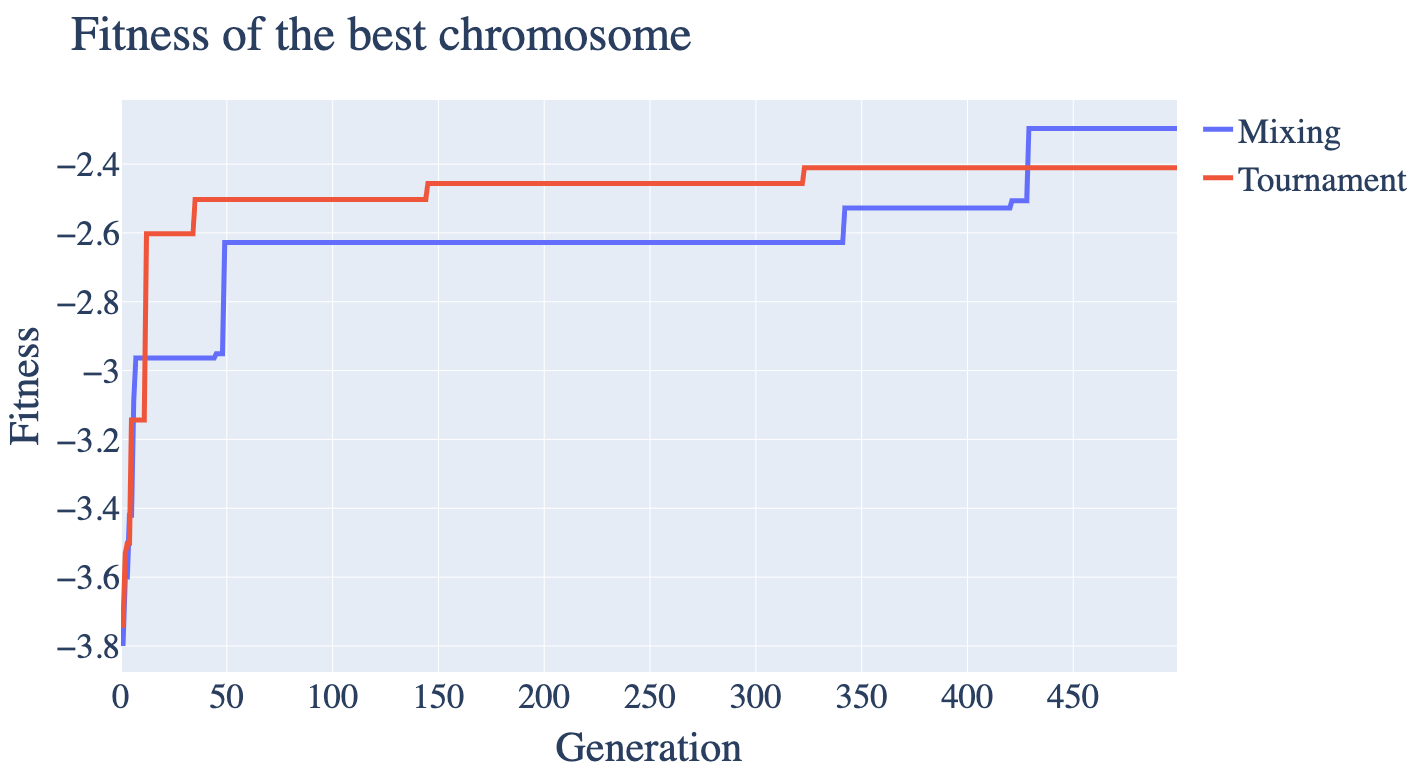
\includegraphics[width=\linewidth]{gen_top_default.png}
    \endminipage\hfill
    \minipage{0.49\textwidth}
    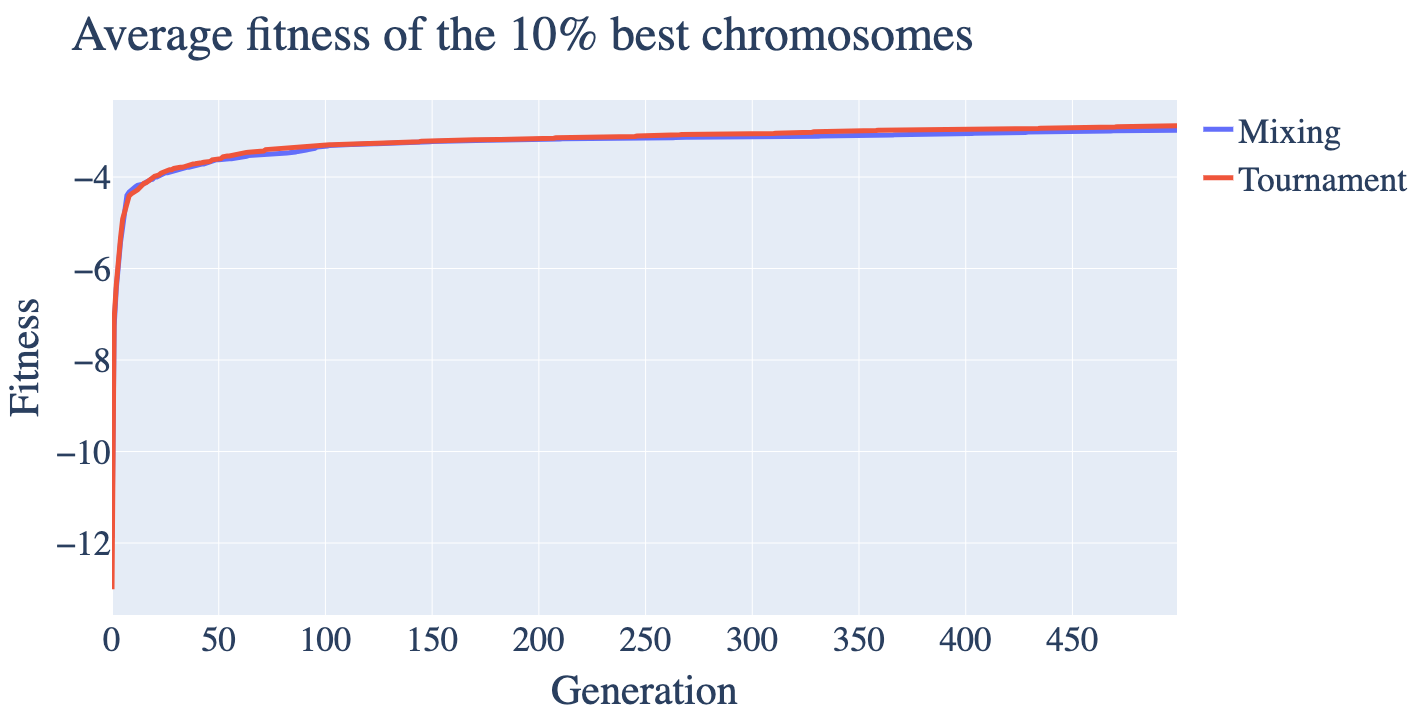
\includegraphics[width=\linewidth]{gen_10_default.png}
    \endminipage\hfill
    \minipage{0.49\textwidth}
    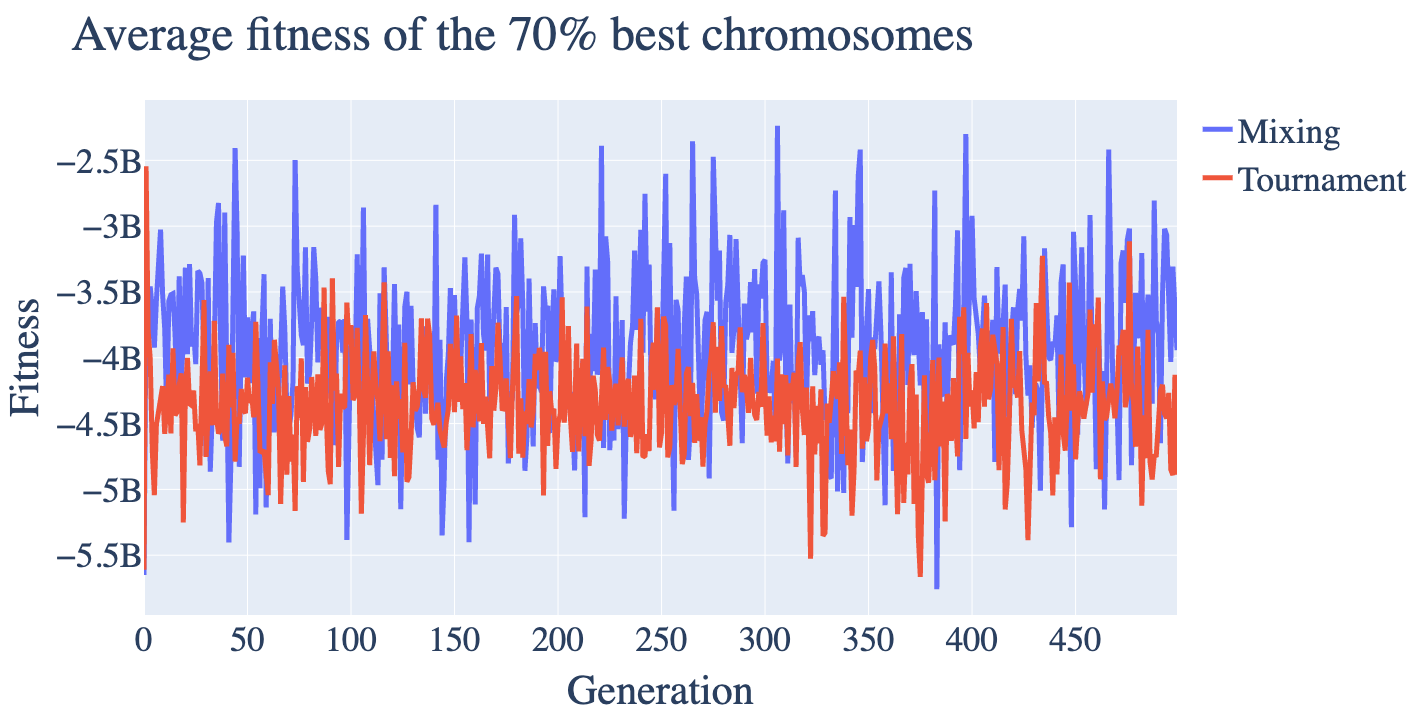
\includegraphics[width=\linewidth]{gen_70_default.png}
    \endminipage
    \caption{Three plots showing the fitness of the top chromosome, the average fitness of the 10 \% best chromosomes and the 70 \% best chromosomes respectively, using mixing and tournament selection.}
    \label{fig:gen_default}
\end{figure}


\begin{figure}[h]
    \minipage{0.49\textwidth}
    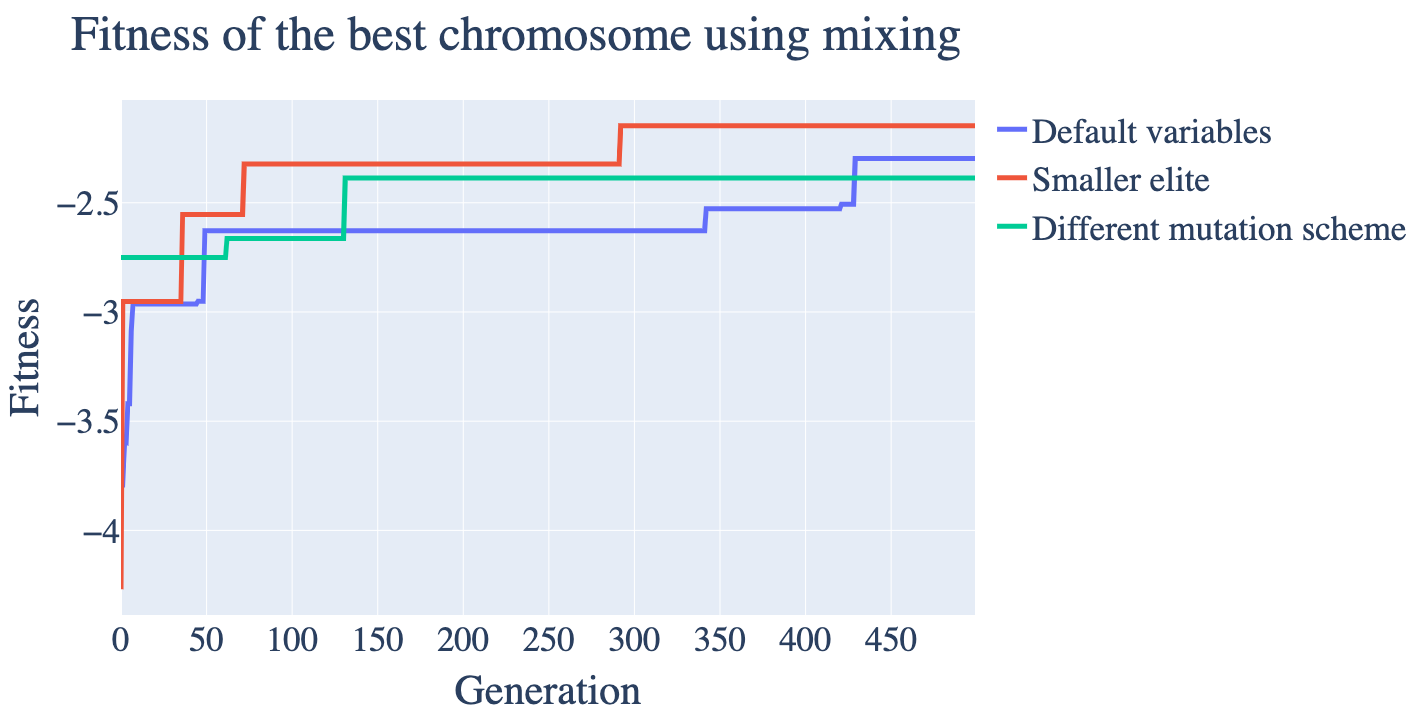
\includegraphics[width=\linewidth]{gen_mix_var.png}
    \endminipage\hfill
    \minipage{0.49\textwidth}
    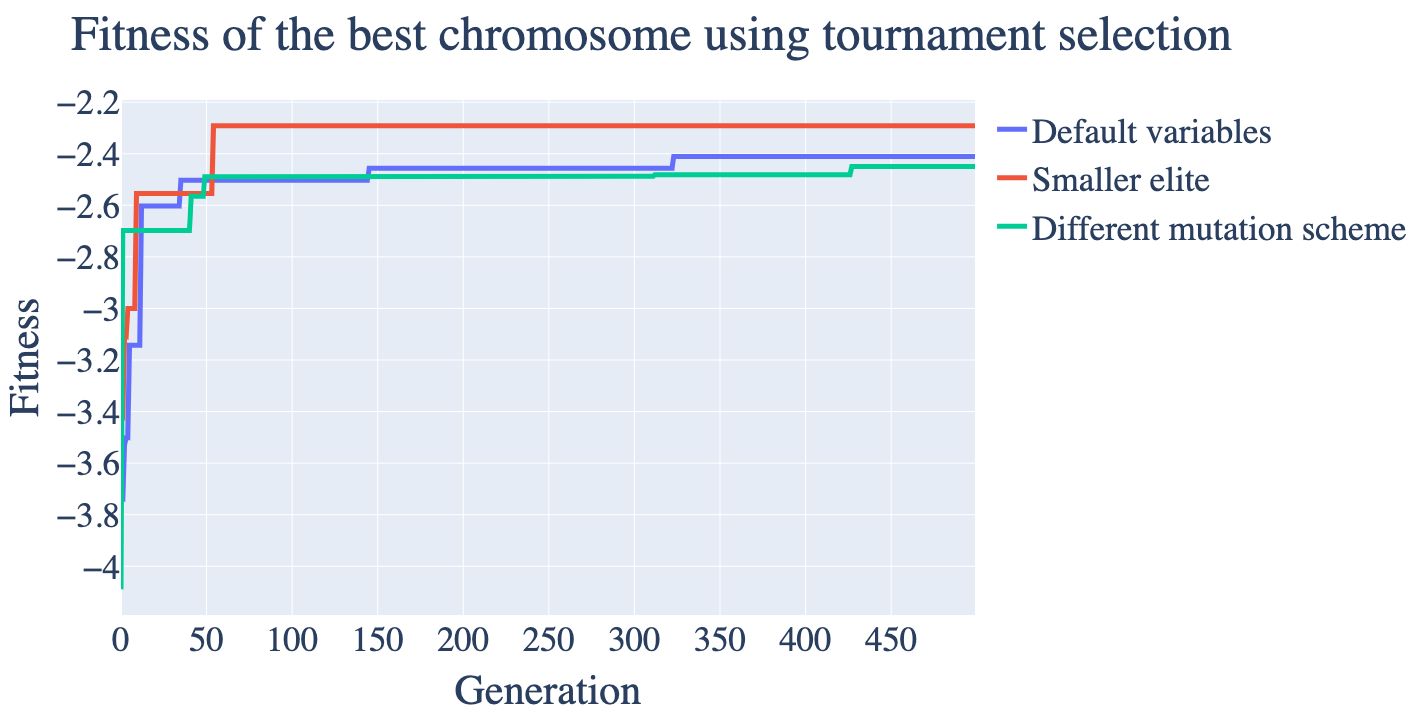
\includegraphics[width=\linewidth]{gen_tour_var.png}
    \endminipage
    \caption{Plots of the fitness of the top gene as function of generations using slightly different variables, using mixing (upper plot) and tournament selection (lower plot).}
    \label{fig:gen_var}
\end{figure}

\begin{figure}[h]
    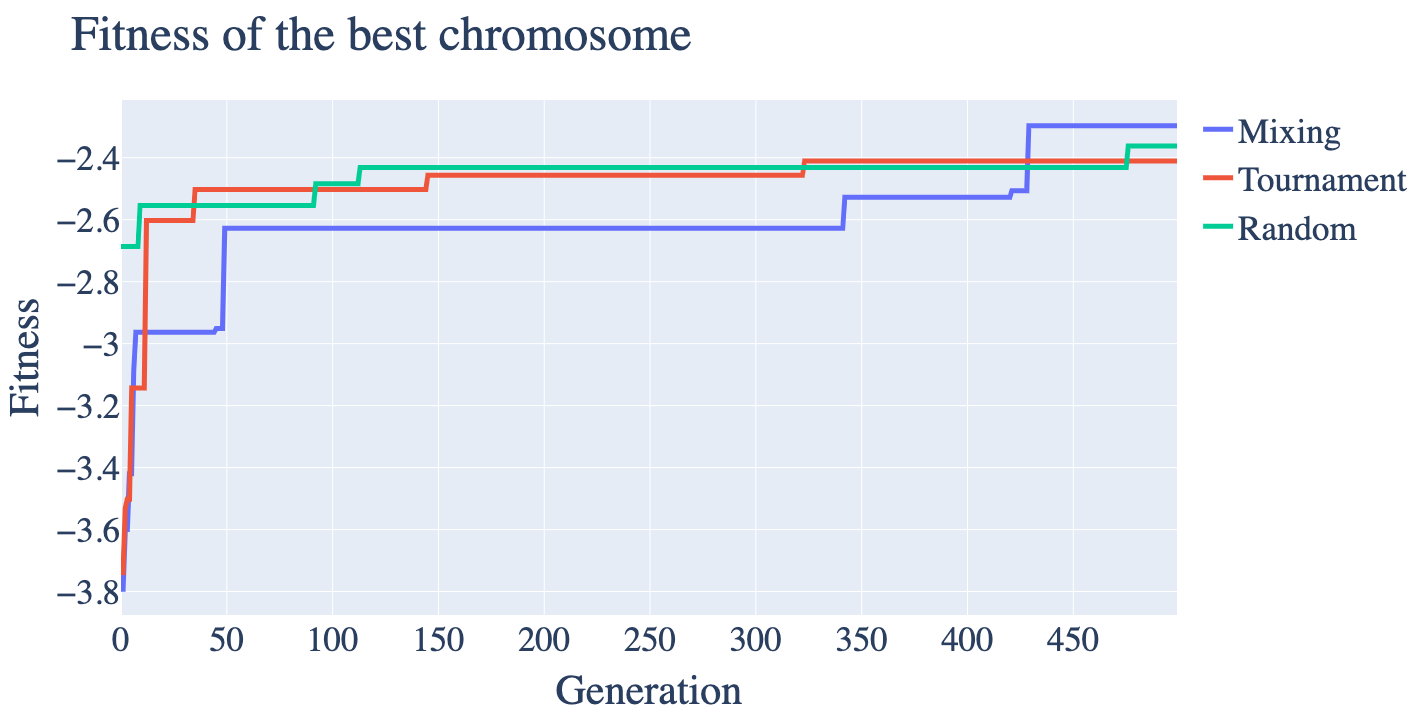
\includegraphics[width=\linewidth]{gen_top_random.png}
    \caption{Plot of the fitness of the top gene as function of generations for the three different selection and crossover methods.}
    \label{fig:gen_random}
\end{figure}

It was then attempted to independently change some of the other variables, namely the size of the elite group and the mutation rate. First, the size of the elite group was decreased to 5 \%. Secondly, the size of the elite group was set back to 10 \%, but the mutation scheme was changed. Instead of applying mutations to 10 genes in half of the new chromosomes, 3 genes were changed in all of the new chromosomes. This resulted in three different methods, and the fitness of the best chromosome over the generations using the different methods using mixing and tournament selection are shown in Figure  \ref{fig:gen_var}. 


In sum, the genetic algorithm employed successfully reproduces the results from \cite{Lagaris}, where fairly simple analytic expressions are found which fulfil the differential equation and the boundary conditions. However, large populations (1000 chromosomes) and many generations are needed before the desired results are obtained, and importantly, it is far from clear that these are found through cumulative selection, and not just by chance. Looking at the plots of the fitness of the fittest chromosome over the generations, it is clear that this tends to increase step-wise, rather than through a slow process of cumulative selection, which is the process the genetic algorithms are aiming to recreate. This should therefore be a source of worry. In fact, when analysing the algorithm of grammatical evolution employed, it is not surprising that there are few signs of cumulative selection in the results, for it is hard to see how the algorithm would be able to recreate this feature of evolution. To understand why, one must go back to the building block hypothesis and the notion of fitness landscapes. These ideas express two necessary conditions for evolution to take place which also apply to genetic algorithms. Firstly, as stated by the building-block hypothesis, the optimal solution must be built up from independent contributions from different building blocks, as encoded in the genes. Secondly, the fitness landscape expresses the requirement that evolution must be cumulative, such that small changes to the genotype (e.g. changing a few genes) does not normally lead to dramatic changes in the phenotype (here the resulting function). With the above grammar and algorithm used, however, neither requirement is met.

To understand why, it might be useful to look at an example of two sets of genes, [0, 2, 0, 4, 2, 5, 7, 3, 6, 8, 9, 2] and [0, 0, 0, 4, 2, 5, 7, 3, 6, 8, 9, 2]. The only difference in the genotype is the second gene, but whereas the first leads to the expression $sin(x)t$, the second gives the expression $\frac{xt}{6} + 2$. Thus, changing a single gene completely changes the expression generated, making gradual improvements to the expression by changing individual genes near impossible.

<<<<<<< HEAD
One of the main problems with the grammar used, and how it becomes disanalogous with the process of natural selection, is in the dependence on the preceding genes in the interpretation of the current gene. In other words, the genes found at the different loci (positions in the genetic sequence) do not have any meaning independent of the genes found at the other loci. This breaks with the underlying assumption justifying the selection and crossover operations, where it is assumed that individual genes contribute to the fitness of the individual and are therefore ``good'' or ``bad'', such that mixing the genes of two fit individuals will give another fit individual. However, when this operation is performed using the above decoding scheme, the meaning of individual genes is completely changed by the change in the preceding genes, so the justification for the entire crossover-scheme breaks down. Thus, the structure of the analytical expressions is rarely preserved during crossover, especially not when the genes are mixed perfectly. Thus, the above algorithm seems to mostly work through brute force by guessing at a very high number of candidate solutions and preserving the best ones from each generation. With 1000 chromosomes and 1000 generations, it is far from surprising the the correct solution eventually pops up by chance, provided this is not too complicated. This means that generating new genes at random instead of using a selection process should give similar results, as long at the ``elite'' is still passed on unaltered over the generations. Note that this is only expected to give similar results for the top chromosome - completely replacing the remaining 90 \% of the population every generation will likely give a worse average fitness. 

To test this assumption, a third random selection scheme was introduced. Here, after passing on the elite, consisting of the 10 \% best chromosomes, the remaining 90 \% were generated using the same random method as was used in the first generation when the chromosomes were first initialised. A comparison of the three methods is shows in Figure \ref{fig:gen_random}. 
=======
One of the main problems with the grammar used, and how it becomes disanalogous with the process of natural selection, is in the dependence on the preceding genes in the interpretation of the current gene. In other words, the genes found at the different loci (positions in the genetic sequence) do not have any meaning independent of the genes found at the other loci. This breaks with the underlying assumption justifying the selection and crossover operations, where it is assumed that individual genes contribute to the fitness of the individual and are therefore ``good'' or ``bad'', such that mixing the genes of two fit individuals will give another fit individual. However, when this operation is performed using the above decoding scheme, the meaning of individual genes is completely changed by the change in the preceding genes, so the justification for the entire crossover-scheme breaks down. Thus, the structure of the analytical expressions is rarely preserved during crossover, especially not when the genes are mixed perfectly. Thus, the above algorithm seems to mostly work through brute force by guessing at a very high number of candidate solutions and preserving the best ones from each generation. With 1000 chromosomes and 1000 generations, it is far from surprising the the correct solution eventually pops up by chance, provided this is not too complicated. This means that generating new genes at random instead of using a selection process should give similar results, as long at the ``elite'' is still passed on unaltered over the generations. Note that this is only expected to give similar results for the top chromosome - completely replacing the remaining 95 \% of the population every generation will likely give a worse average fitness.

To test this assumption, a XXX third random selection scheme was introduced. Here,
>>>>>>> 2e9f56d81d316cfb65920742fe7589e0a5f3b271

Why do we find the simple solutions but not this one? Because it is very unlikely for the complete solution to come up by chance, given how long it is. 

This is, however, very far from the intended mechanism with which the genetic algorithm is meant to work, and to call it machine learning is simply wrong. To improve it, a different encoding scheme would be needed for the genetic code, one which gives each locus in the genome an unambiguous interpretation, independent of the other genes. This would preserve the structure of the expressions between mutations, and would allow for small, step-wise adaptations. The development of such an encoding scheme, however, is far beyond the scope of this paper.


\section{Conclusion}

\bibliographystyle{plain}
\bibliography{refs}

\end{document}
